\documentclass{article}
\usepackage{amsmath}
\usepackage{tikz}
\usetikzlibrary{patterns}

\begin{document}

\begin{figure}[h]
    \centering
    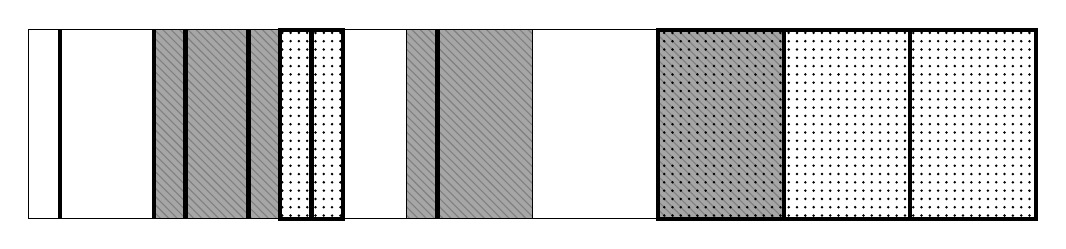
\begin{tikzpicture}[scale=0.8]
        % Define the agent's valuation buckets
        \foreach \x in {0,...,5} {
            \draw[fill=gray!70] (\x*2-0.5, 0) rectangle (\x*2+1.5, 3);
            \draw[pattern=north west lines, pattern color=black!50] (\x*2-0.5, 0) rectangle (\x*2+1.5, 3);
        }
        
        % Define the mechanism's query buckets
        \foreach \x in {0, 2, 4} {
            \draw[fill=white] (\x*2-0.5, 0) rectangle (\x*2+1.5, 3);
        }
        
        % Draw the black boxes indicating the alternative chosen by the mechanism
        \draw[ultra thick, pattern=dots, pattern color=black] (3.5, 0) rectangle (4.5, 3);
        
        % Draw the black boxes indicating the alternative chosen by the mechanism
        \foreach \x in {5, 6, 7} {
            \draw[ultra thick, pattern=dots, pattern color=black] (\x*2-0.5, 0) rectangle (\x*2+1.5, 3);
        }
        
        % Draw the lines between the buckets
        \draw[ultra thick, pattern=dots, pattern color=black] (0, 0) -- (0, 3);
        \draw[ultra thick, pattern=dots, pattern color=black] (2, 0) -- (2, 3);
        \draw[ultra thick, pattern=dots, pattern color=black] (4, 0) -- (4, 3);
        \draw[ultra thick, pattern=dots, pattern color=black] (6, 0) -- (6, 3);
        
        % Define the alternative's ranking
        \draw[ultra thick, pattern=dots, pattern color=black] (0, 0) -- (0, 3);
        \draw[ultra thick, pattern=dots, pattern color=black] (1.5, 0) -- (1.5, 3);
        \draw[ultra thick, pattern=dots, pattern color=black] (3, 0) -- (3, 3);
        \draw[ultra thick, pattern=dots, pattern color=black] (4.5, 0) -- (4.5, 3);
    \end{tikzpicture}
    \caption{An example for our lower bound construction in Theorem~\ref{thm:omega_log_m_lower_bound_non_stochastic}. The black boxes indicate the alternative $\widehat{a}$ picked by the mechanism $\mathcal{M}$ in each agent's ranking. The mechanism queries the positions corresponding to the dashed boxes. In this example, the mechanism only queries the first position in a bucket, which is without loss of generality. The gray areas correspond to buckets where all alternatives have high values, while white areas correspond to buckets where alternatives have low values, either because the bucket contains the winning alternative $\widehat{a}$ or because the mechanism queries the value of an alternative in the bucket.}
    \label{fig:omega_log_m_lower_bound_example}
\end{figure}

\end{document}